\subsection{viertes}

\begin{comment}
  zula Barbara Seite 46
\end{comment}

\begin{comment}
  Original aus der Zula:
  \[
    P_d=-3t^{14}\partial_t^6+t^{11}(t+3)\partial_t^5 + 2t^8\partial_t^4
    -t^6(t^3+1)\partial_t^3 + t^4\partial_t
  \]

  $ P_d \Rightarrow
  \begin{cases}
    k=6,l=14 & \Rightarrow u\leq k=6, v\geq l-k=8\\
    k=5,l=12 & \Rightarrow u\leq 5, v\geq 7\\
    k=5,l=11 & \Rightarrow u\leq 5, v\geq 6\\
    k=4,l=8 & \Rightarrow u\leq 4, v\geq 4\\
    k=3,l=9 & \Rightarrow u\leq 3, v\geq 6\\
    k=3,l=6 & \Rightarrow u\leq 3, v\geq 3\\
    k=1,l=4 & \Rightarrow u\leq 1, v\geq 3\\
  \end{cases} $

  also ist Abbildung 5.8 auf seite 53 der zula falsch?
\end{comment}

\[
  P_d=-3t^{14}\partial_t^6+t^{11}(t+3)\partial_t^5 + 2t^8\partial_t^4
  -t^6(t^3+1)\partial_t^3 + t^3\partial_t
\]

$ P_d \Rightarrow
\begin{cases}
  k=6,l=14 & \Rightarrow u\leq k=6, v\geq l-k=8\\
  k=5,l=12 & \Rightarrow u\leq 5, v\geq 7\\
  k=5,l=11 & \Rightarrow u\leq 5, v\geq 6\\
  k=4,l=8 & \Rightarrow u\leq 4, v\geq 4\\
  k=3,l=9 & \Rightarrow u\leq 3, v\geq 6\\
  k=3,l=6 & \Rightarrow u\leq 3, v\geq 3\\
  k=1,l=3 & \Rightarrow u\leq 1, v\geq 2\\
\end{cases} $

\begin{center}
  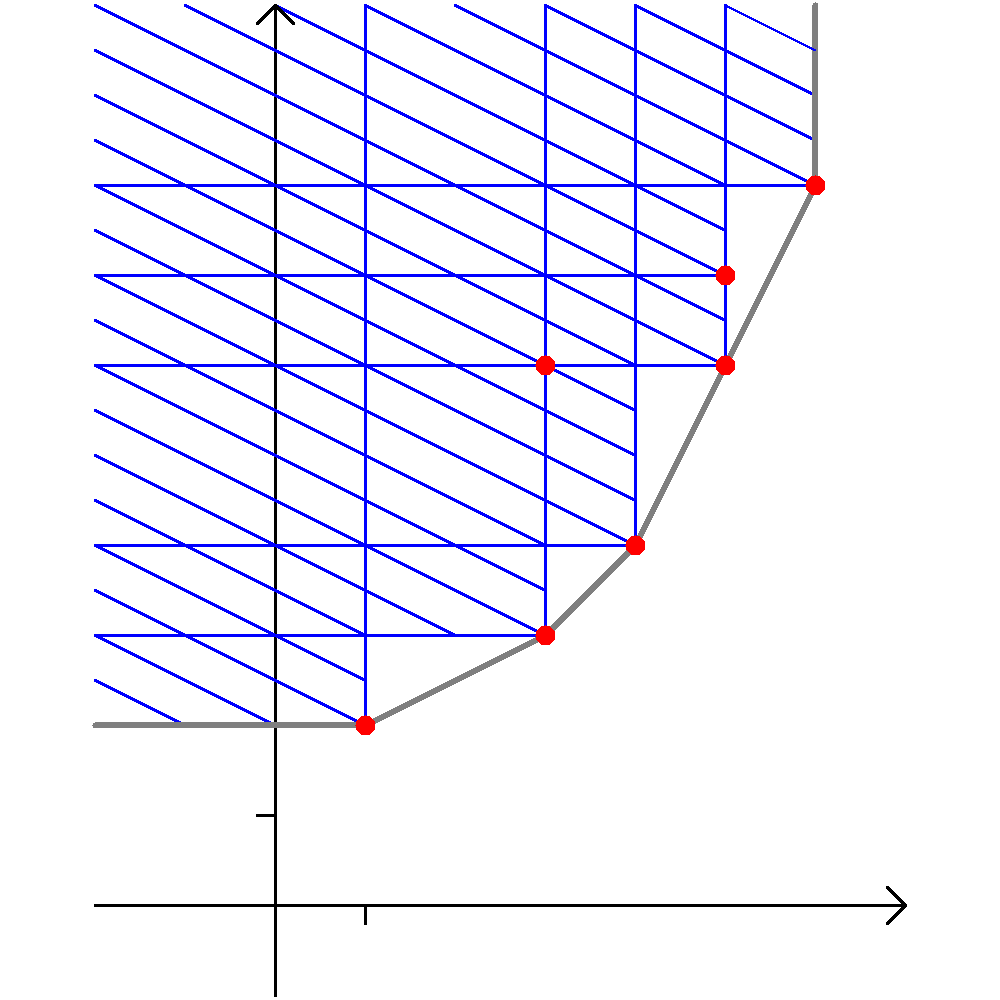
\includegraphics[width=6cm]{beispiele/img/d.png}
\end{center}
also $\slopes(P_b)=\{0,\frac{1}{2},1,2\}$ also ist $P_d$ irregulär singulär.\\
Offenbar ist der Hauptnenner der Steigugnen gleich $2$.\\
Betrachte also $\rho:t\mapsto u^2$\\
und erhalte: ???

% vim: set ft=tex :
